\documentclass[conference]{IEEEtran}
\usepackage{graphicx}
\usepackage{amsmath}
\usepackage{enumerate}
\usepackage{multirow}
\usepackage{epstopdf}
\usepackage{array}
\usepackage{CJK}
\usepackage{float}
\usepackage{subfigure}
\usepackage{algorithm}
\usepackage{algorithmicx}
\usepackage{balance}
\newcommand{\algorithmicbreak}{\textbf{break}}
\newcommand{\BREAK}{\State \algorithmicbreak}
\usepackage{algpseudocode}

\hyphenation{op-tical net-works semi-conduc-tor}


\begin{document}

\title{OnCampus: A Scheme Towards Smart Campus}


% author names and affiliations
% use a multiple column layout for up to three different
% affiliations
\author{\IEEEauthorblockN{Zhen Chen, Jialiang Kang}
\IEEEauthorblockA{School of Software, Dalian University of Technology, Dalian 116620, China\\
f.xia@ieee.org}}

% conference papers do not typically use \thanks and this command
% is locked out in conference mode. If really needed, such as for
% the acknowledgment of grants, issue a \IEEEoverridecommandlockouts
% after \documentclass

% for over three affiliations, or if they all won't fit within the width
% of the page, use this alternative format:
%
%\author{\IEEEauthorblockN{Michael Shell\IEEEauthorrefmark{1},
%Homer Simpson\IEEEauthorrefmark{2},
%James Kirk\IEEEauthorrefmark{3},
%Montgomery Scott\IEEEauthorrefmark{3} and
%Eldon Tyrell\IEEEauthorrefmark{4}}
%\IEEEauthorblockA{\IEEEauthorrefmark{1}School of Electrical and Computer Engineering\\
%Georgia Institute of Technology,
%Atlanta, Georgia 30332--0250\\ Email: see http://www.michaelshell.org/contact.html}
%\IEEEauthorblockA{\IEEEauthorrefmark{2}Twentieth Century Fox, Springfield, USA\\
%Email: homer@thesimpsons.com}
%\IEEEauthorblockA{\IEEEauthorrefmark{3}Starfleet Academy, San Francisco, California 96678-2391\\
%Telephone: (800) 555--1212, Fax: (888) 555--1212}
%\IEEEauthorblockA{\IEEEauthorrefmark{4}Tyrell Inc., 123 Replicant Street, Los Angeles, California 90210--4321}}

% make the title area
\maketitle


\begin{abstract}
With the development of information technology, an increasing number of researchers and engineers begin to work on constructing smart city. As an important component of smart city construction, college campus has also been paid much attention. How to construct smart campus becomes a topical issue. In this work, we propose a scheme to assist building a smarter and more friendly campus. We focus on three aspects towards smart campus: discovering social circles based on interests mining, providing educational guidance by emotion analysis on an information posting platform, and developing a secondary trading platform aiming at campus resources allocation optimization. Based on the three aspects, we implement a prototype called OnCampus as the first step of smart campus construction, which has been practiced in Dalian University of Technology. The aforesaid three purposes of smart campus can be well achieved by OnCampus.
\end{abstract}

% For peer review papers, you can put extra information on the cover
% page as needed:
% \ifCLASSOPTIONpeerreview
% \begin{center} \bfseries EDICS Category: 3-BBND \end{center}
% \fi
%
% For peerreview papers, this IEEEtran command inserts a page break and
% creates the second title. It will be ignored for other modes.
\IEEEpeerreviewmaketitle



\section{Introduction}

%The construction of smart campus under the background of smart city
Information technology has brought tremendous changes to our lifestyle and living environment, which is reflected in daily livelihood,  communication, public security, energy, water resource etc. Comprised with pervasive networks, advanced electronics, various sensors, urban is evolving to be smart city. Smart city is defined as "multiple sectors cooperating to achieve sustainable outcomes through the analysis of contextual real-time information shared among sector-specific information and operational technology systems"~\cite{szabo2013framework}. Many researches contribute to smart traffic system, smart medical system, smart food system to support smart city. As a special epitome of society, college campus is a significant component element of city.

%development of mobile deveces and liked by college student
As far as we know, mobile devices perform to be an ideal assistant platform to improve the efficiency of campus life~\cite{chen2012oncampus}. Since they are portable and easily accessible, they have become a necessary part of millions of college students in their daily life. Recent years, Mobile devices are being widely applied in the campus scene. For instance, Mobile Virtual Campus (MVC)~\cite{tan2010collaborative} and T3G~\cite{chu2010two} are two useful mobile learning tools for college students. Meanwhile, it is noticed that location based service (LBS) has brought much improvement for mobile living experience with more precise and reliable service~\cite{zhao2012mobimsg}. College students are always fascinated by these advanced technologies, especially smart phones. Studies have shown that the increasing  smart phones within college campus are accessing to the Internet at an overwhelming speed. As a consequence, mobile platforms and its' location based service seem to be important factors when considering smart campus.

%We regard college campus as a domain after analysis and consideration of its characteristic
College campus can be summarized to be a scene: a well-organized area containing high quality infrastructure, full of students' personal information and education resources, being students' long-time living place. Under such conditions, smart campus is desired to be like this: 1) More accurate context awareness and ubiquitous access to network. 2) Resources are allocated efficiently. 3) Decisions are made smartly based on revealing the objective principles. 4) Students can easily establish or enhance friendships based on intersecting circles. As well as students' freedom of speech can be protected. However, there is a huge gap between this wonderful vision and the current progress on building smart campus. There have been much attempts towards smart campus that focus on physical campus infrastructure and virtual intelligent services. Although many campus contexts are taken into account, most work concentrate on physical equipments or functional applications. In our opinion, paralleled development of either physical or virtual campus services is no better than an effective interweaving to constructing smart campus. Thus, we innovatively propose a scheme supporting smart campus by utilizing some theoretical concepts and academic approaches, such as interests mining, recommendation technology and educational guiding model. Based on the scheme, we design and implement an architecture to offer intelligent services. Our objectives are making campus a smarter and more friendly place to live.

%needs and our solution
In this work, we mainly make contributions on three aspects. 1) Introduce interests mining models based on the context awareness, locations, students profiles and relationships. Establish interests circles based on this.  2) Provide a platform on which users can share knowledge, post ideas, ask or answer questions. Managers can collect and analyze students posts, aimed at analyzing "campus emotion" and provide appropriate educational guiding. 3) Devote to optimizing the campus resources, such as used books, surplus products etc. We design and developed a system called OnCampus based on mobile devices to support smart campus.

The rest of this paper will be developed as follows. Section II introduces the state of art of the research of smart campus, as well as researches about interests mining. Section III presents our motivation and requirements for smart campus, including personalized service, scientific guidance and resources optimizing. And the following section IV has discussed the scheme we proposed towards constructing smart campus. With the knowledge of our scheme, in section V we design and implement a prototype for both client side on mobile phones and server side on PCs. Finally, section VI gives a conclusion about our work.

\section{Related Work}

The idea of smart campus are not new. On the way of constructing smart campus, more attentions are remained on the infrastructures and the related applications involving both learning and teaching as well as living guidance in order to promote personal experience.

%campus learning %education perspective
Smart campus are often approached from educational and learning perspective. In 2010, A new paradigm of thinking pertaining to a novel holistic intelligent campus (iCampus~\cite{ng2010intelligent}) environment is proposed in order to enrich the end-to-end learning lifecycle of a knowledge ecosystem. Atif et al.~\cite{atif2013social} propose a smart campus model, which integrates real-world learning resources in a campus-wide social network. This model aims to situate learners in a smart campus environment that provides context-based personalized learning and feedback. Hirsch et al.~\cite{hirsch2011education} propose mobile cloud education as a ubiquitous, cloud-based way of providing anytime-anywhere context-aware learning using portable devices. Liu et al.~\cite{liu2014research} also consider smart campus to be an inevitable trend in the development of digital campus construction. They expound the concepts of smart campus based on the cloud computing and internet of things, and discuss the problems should be noticed after elaborating intelligent application platforms.

%campus on data analysis
Many researchers also devote to building smart campus based on data analysis. Adamko et al.~\cite{adamko2014system} aim to establish an intelligent campus which is based on gathering data from the crowd, analyze them and provide feedback as value-added services that make users glad and in the meantime contributory as they would like to return. Boran et al.~\cite{boran2011smart} describe the implementation of a Smart Campus application prototype that integrates heterogeneous data using semantic technologies. Some work also contributes to smart campus in social networking aspect. Yu et al.~\cite{yu2011towards} develop a system architecture based on the service-oriented specification to support social interactions in campus-wide environments. Xiang et al.~\cite{xiang2015smart} discuss the features and functions of a social network platform, WeChat, and put forward a smart university campus information dissemination framework based on the WeChat platform.

%energy ef?ciency point of view
Many of the initiatives~\footnote{http://greensmartcampus.eu/} \footnote{http://smartgridcenter.tamu.edu/seci/} think primarily of smart campus from an energy high-efficiency point of view. Zhao et al.~\cite{zhao2012mobimsg} propose a resource-efficient location-based mobile instant messaging system which is used in smart campus situation. Yim et al.~\cite{yim2014design} design and implement a VOD(video on demand) system, which is a smart campus guide android App that recognizes the structure in which a user is interested and displays useful information about the structure.

Although practical in each individual area, these projects work in very limited ways, either drawing a map of the campus or presenting e-books. None of them present the colorful campus life as a versatile system to assist college students, offering efficiency and convenience.

Researchers who are major in interests mining conduct their researches mainly on topic model on web text, like blog or Microblog. Nearly little researches focus on interests mining in campus environment. Kuang et al.~\cite{kuang2010user} build an exact model for user interests by users�� log and users�� learning condition from an e-learning system, so that they can automatically identify the learner��s interests and recommend interest-related resources. Han et al.~\cite{han2014data} conduct their research on Web log mining and propose a data preprocessing method based on user characteristic of interests and show the superiority and recommended value of this new method. Chen et al.~\cite{huayue2012study} use topic model to build up users�� interest model, based on which they can provide resource recommendation for users in the system.

Although researchers are sparing no effort exploring the construction of smart campus, of which the development seems to be still at the primary stage. Some researchers analyzed the characteristics and trend of smart campus, reminding the problems need to be paid attention in the process of constructing smart campus. The state of art of achievements seem to lie mainly in the construction of infrastructure and service application. Some others attempt on improving the security or efficiency of campus life via cloud computing and internet of things. These efforts benefit users from a substantial but relatively restricted way like navigation service. Our work means to contribute to establishing smart campus, and propose an efficient scheme composed of interests mining, resources optimizing and scientific guiding. In the scheme we propose a new concept, campus emotion, to offer a better personal experience of campus life for college students.

\section{ Motivations and Requirements}

%We regard college campus as a domain after analysis and consideration of its characteristic
College campus can be summarized to be a environment where not only does it provide good infrastructure and condition to conduct context-aware services, but also it is a well-organized area within which a substantial number of user spends majority of time and generates a huge number of information or needs. These information is directly related to context of campus, such as location, user profiles, etc. Smart campus is desired to be more accurate context awareness and ubiquitous access to network, and tremendous resources are optimized efficiently and predictions or decisions are made smartly based on the objective principles. We aim to serve college students a versatile and talented campus experience, meanwhile giving a practical hand on campus life. What we are going to do is to provide a feasible scheme for satisfying their requirements, thus facilitating the contribution of smart campus means an efficient and convenient college life.

%needs and our solution
College student, generally, they spend time on the communication with families, friends, and even strangers, to establish or enhance friendships. But unfortunately, in most cases, students may have no way to access what they want or even develop their other interests. Interests mining based on the context awareness, locations, user profiles and proximity, and other information can facilitate college students satisfying their needs and making the most of resources in school. Particularly, wise decision and prediction can be made for faculty if they have a perception of the mood trend of the students who can get more scientific and efficient guidance.

The following scenario illustrates the requirements to be satisfied towards smart campus:

With great passion and curiosity, Bob entered the university dreaming a colourful college life. In campus environment, students, researchers and many other entities performed various activities. Facing the mass information of the multifarious social activities displayed, he felt at sea because he didn't know what he was really interested in. Under the urge of his great passion, he chose some social activities and clubs to take part in because of the participated students surrounding him. However he left the clubs because it was proven to be not accord with his interest after a period of time. The same embarrassment occurred when he chose his profession one year later, but this time he could NOT leave. No longer did he have the passion or desire to try new things. He found it really difficult to conduct his exploration on his research without a cooperator.

One day, he took part in a demonstration against the school institution because of the invitation and complainants which he took for granted from his roommate who had decided to demonstrate for the same reason. When he graduated, he had to throw away some articles for daily use or books which would be useful and helpful for other students.

Bob's experience is the epitome of college experience for most college students currently. We survey students about their daily life to find out students' requirements. Actually, the requirements of university students are diverse and cover their study, living and entertainment. We can submit the requirements shown in Fig. \ref{Fig1:overview} when considering constructing smart campus:

\begin{figure}[htb]
\centering
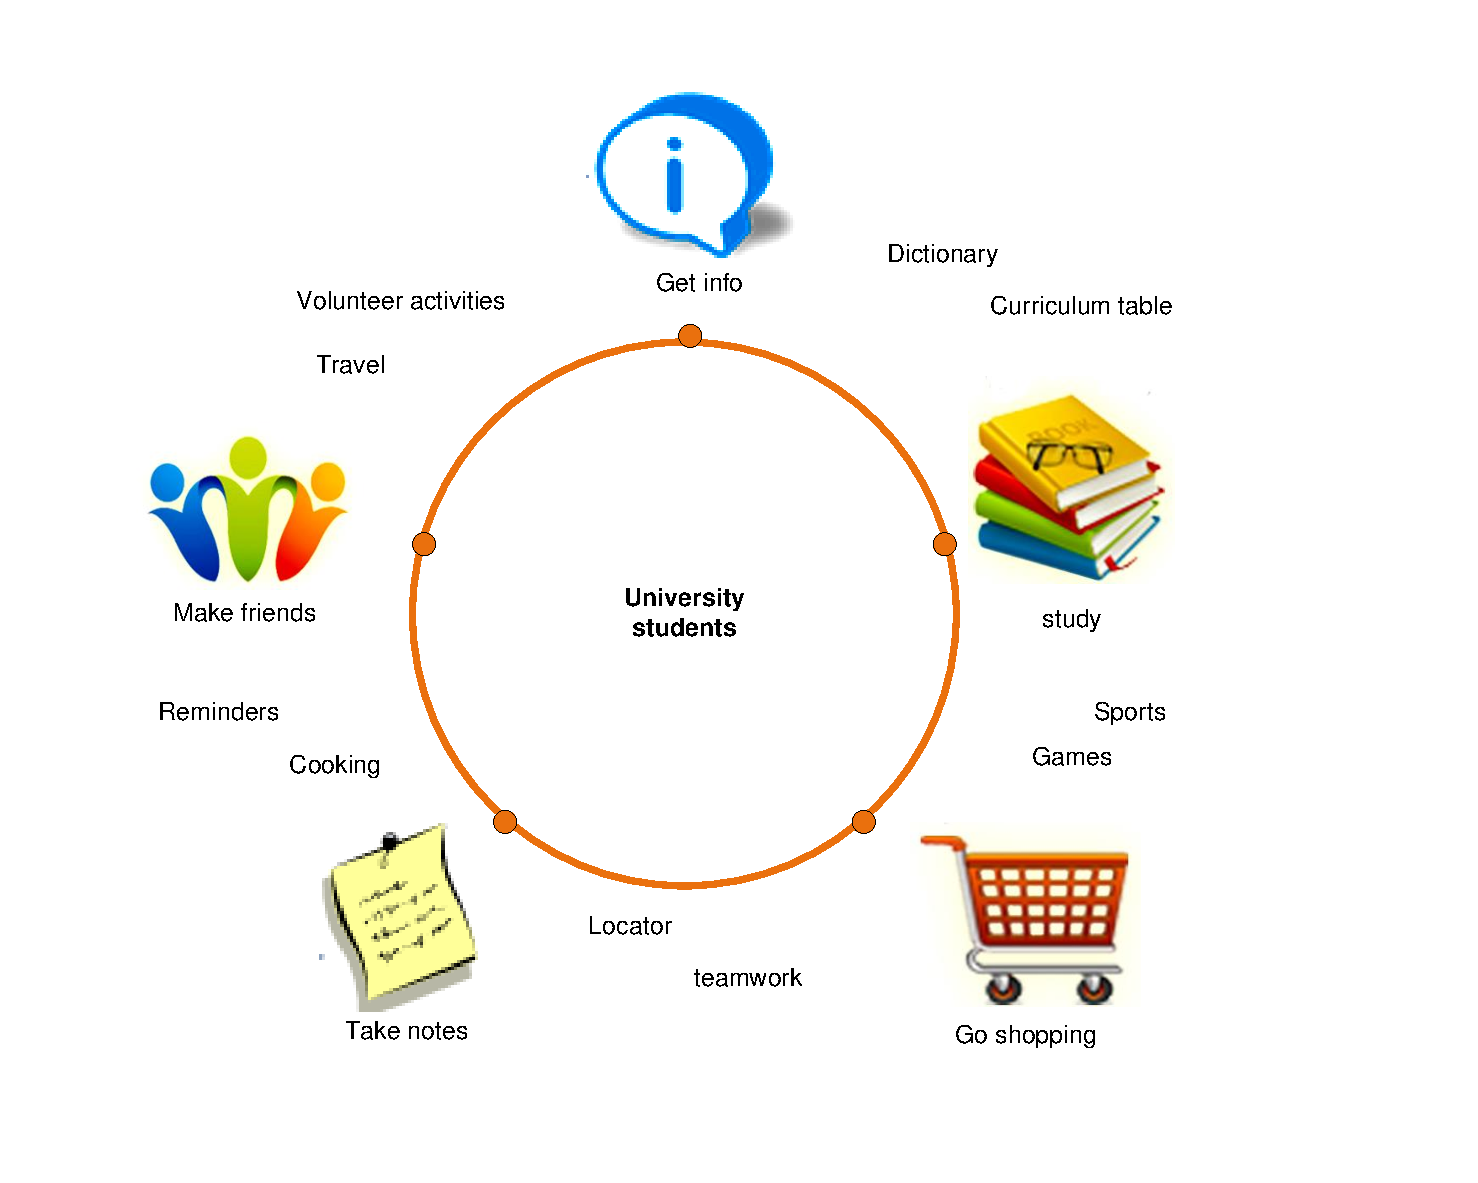
\includegraphics [width=3in]{Fig1.pdf}
\caption{Overview of requirements}
\label{Fig1:overview}
\end{figure}
\begin{enumerate}
  \item Personalized Service. It will be wiser and more beneficial for smart campus to provide information and service depending on the users' interests and profile. Otherwise the information explosion may dispel the enthusiasm of campus actors including students and teachers. Proper recommendation based on interests mining in campus environment will be discussed in next section, which is a very good solution we proposed to offer personalized service.
  \item Scientific Guidance. The community of college students, as a particular group of people, are mostly comprised of enthusiastic youth. Though they are well educated, it is the long time education in school makes them lack of experience or well judgement. Meanwhile, they are eager to make contribution to family and society with great passion. All of these characteristics lead them easily to be cat's paw. In next section, we will introduce our vision of conduct scientific guidance based on predicting the community's behavior and emotion. We also propose the phrase "campus emotion" vividly in our scheme.
  \item Resources Optimizing. The concept of resource in smart campus is not restricted in entity resources. Moreover, the information, context, event and even users themselves, can be particular resource which should be optimized. We are verifying a recommendation algorithm utilizing friendship of the user, which we regard as a solution to resources optimizing.
\end{enumerate}

\section{Proposed Scheme}

%Assumption
In our work, we make following 2 assumptions: 1) Pervasive access to network: we assume that every user such as students, faculties is equipped with a personal device(PC, smart mobile device, PDA etc). In smart campus systems, devices owned by users and the infrastructure form the condition that in campus situation\cite{khabou2014threshold}, users maintain a constant connection with each other, they are benefitted from a pervasive access to network, such as social network, learning network etc. 2) Precise context awareness: it is supposed that the smart campus system has the powerful capability of context awareness and pervasive computing\cite{khan2007future}. Besides the users' profile, the environment users involved in such as building, location will be precisely obtained by advanced context extraction, identification and integration for smart campus.

The scheme we proposed is composed of interests mining, scientific guidance and resources optimizing based on the above assumptions.

As mentioned before, we put interests mining forward into smart campus to offer personalized service from a unique perspective. Different from the state of art interests mining mainly on semantic analysis from web or web behavior. We take campus context into consideration, from information of location, time, frequency, track and accompany, to inferring the users' interests or needs. Then a customized recommendation strategy will filter the explosive information or resources to provide personalized service. For example, if a user appears in library frequently, always reading magazines about astronomy. Users with the similar interest may be recommended. This can be an effective way to find potential friends or cooperators. From another perspective, it is also an example of optimizing the resources in campus environment.

To conduct scientific guidance to students, smart campus should offer faculty the conditions of the students. Based on the analysis of most students context and combined with the technology of public opinions analysis, the prediction of the community behavior and emotion can be conducted. We pick up a new phrase called "campus emotion" to evaluate the state of most students. If the campus emotion is healthy or normal, it represents most students are in a positive mood, but if it presents sick, it means that most students are in negative mood. For example, we can infer the impactive of some students via the technology of public opinions analysis. A customized guidance scheme can be formulated by supervisor.

We pay attention to optimizing resources from various aspects. Besides mining potential resources to users, we are trying new recommendation algorithm to satisfy the needs of users. Recommendations cross different domains can be made under the consideration of friendship, and this work is under tested during which it seems to have a better performance than traditional algorithm.

Towards smart campus, we propose a scheme composed of interests mining, scientific guidance and resources optimizing corresponding to the requirement mentioned before. Based on the assumptions, the scheme is a vision on constructing smart campus. Moreover, we put forward some feasible attempts, some of which is under verifying to be efficient. Based on the scheme, we design and implement a prototype named "OnCampus", which will be elaborated in detail in the next section.
%-------------------------------------------------------------------------end------------------------------------------------------------------------------------%

\section{Prototype Implementation}
The prototype is given a name of "OnCampus" to proclaim our aim to serve college students a versatile and talented campus experience. Fig. \ref{Fig2:architecture} shows architecture of OnCampus. This proposed architecture enables the OnCampus to work as a practically versatile campus assistant, archiving real-time messaging and data transmission.  More than simple clients and servers, this architecture attempts to propose location-based interaction as well as rational communication mechanism. Servers appear a two-tier structure, providing service and storing information. The first tier server is a message sending server, storing the information uploaded by mobile clients and transferring requested data to clients�� functional modules. And the second tier is a location searching server which merely collects location information and acquires clients�� location data by interacting with location service module of clients. Clients include the interface of our OnCampus assistant which interacts with users. A client made of three modules covers important college activities: circle communication, local trading and campus forum. With the introduction of location based service (LBS), OnCampus is favorable for students to establish and enhance friendships, knowledge exchange and affective interaction, buy and sell used goods in a campus flea market.

\begin{figure}[htb]
\centering
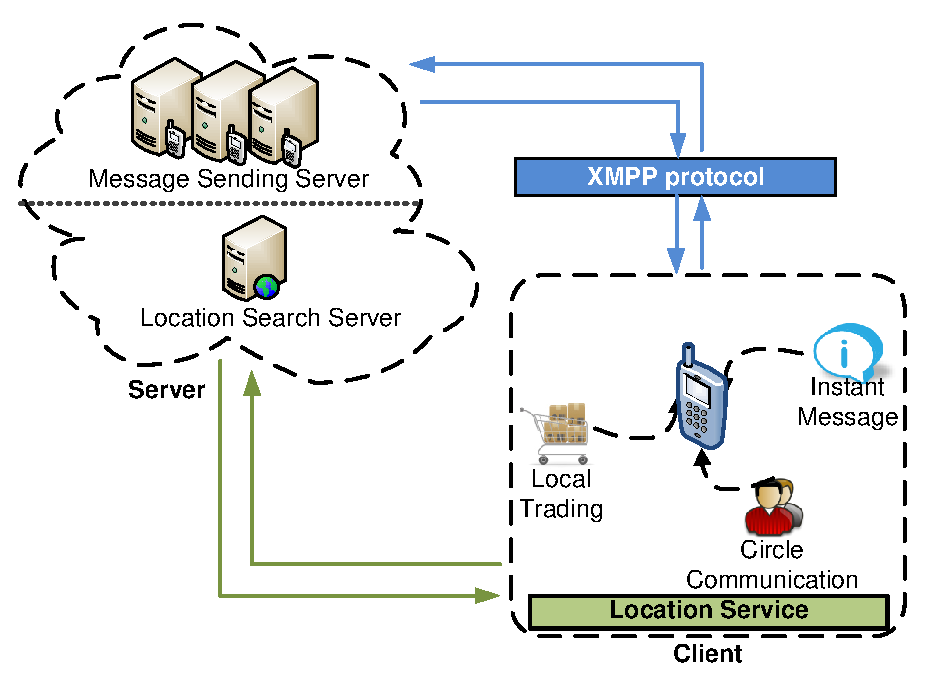
\includegraphics [width=3.5in]{Fig2.pdf}
\caption{Architecture of OnCampus}
\label{Fig2:architecture}
\end{figure}

\subsection{Communication Mechanism}
In the OnCampus architecture, clients communicate with message sending servers on service data and exchange location information with location search servers. This communication via XMPP protocol is quite frequent in order to archive real-time service and data refresh. Data response right coming after each refresh is not adequate concerning energy consumption and network flow. Thus practical communication mechanism is proposed to stipulate data transportation process between servers and clients. This section will further illustrate the structure of server side and discuss the communication process in detail.

\begin{figure}[htb]
\centering
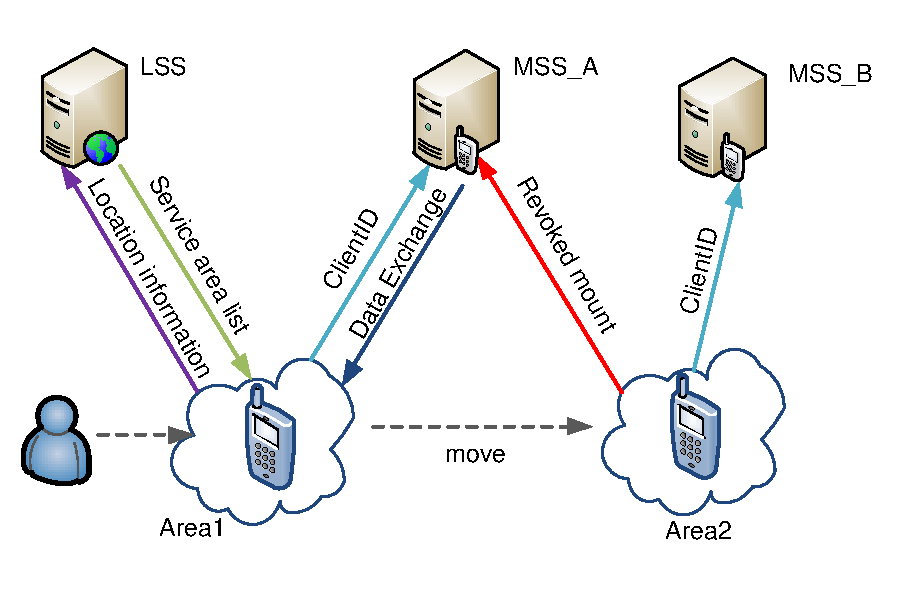
\includegraphics [width=3.5in]{Fig3.pdf}
\caption{Communication process between client and two-tier servers}
\label{Fig3:communication}
\end{figure}

To achieve complicated location service at an energy-saving and efficient way, the OnCampus imposes two-tier server structure, LM2C (Location Search Server and Message Sending Server to Client), as shown in Fig. \ref{Fig3:communication}. And this two-tier structure involves message sending server (MSS) and location search server (LSS). Server side generally is responsible to collect data, classify and group the information automatically, and send messages according to various locations. And separately LSS is the server which manages physical area information and identifies related MSS, but MSS corresponds to store information and broadcast instant messages. Geological partitions are set by LSS, such as Teaching Building 1, Teaching Building 2 and Stadium M, and each physical area ID and its serving scope are documented as attributes of serving areas. With the database of serving areas, it is easy to check out that a certain physical location is assigned to a particular serving area, relating serving areas to a specified MSS. An MSS is in charge of several areas, and maintains a dynamical user list according to the users�� locations. MSSs accomplish the task to broadcast location-based instant messages, treating each physical area specifically.

On the basis of LM2C of server side, OnCampus architecture regulates the process of data transfer between servers and clients to support system service. The communication process of location-based instant messaging between clients and two-tier servers can be illustrated as Fig. 3. When a client connects with LSS, it submits location information to LSS. LSS then will feedback a set of data, including surrounding area attributes, identifiers of MSSs as well as the corresponding relations of connection permission. After receiving the data, client needs to check out which MSS it belongs to, and then client waits for permission from MSS.  MSS adds that client to broadcast list and deliver permission information to client. A message will only be pushed to the clients who are marked in the user list of specified MSS. When this client ranges out of the area of former MSS, the connection between client and former MSS will be dismissed and connection request will be asked to another MSS without communicates with LSS.

This two-tier LM2C architecture is designed to realize location-based instant message push, as well as energy efficiency. As mentioned above, client will receive a set of areas but not one attribute related to its exact location. This is designed for irredundant connection to LSS when location changes, clients decide the next MSS according to given datasets. Thus, an efficient way is implemented on the OnCampus system to use resource and bandwidth for servers. Besides, OnCampus supports that clients can passively receive messages rather than initiatively obtain messages, reducing energy consumption for clients.

\subsection{OnCampus at a Glance}

OnCampus, whether its architecture with the use of location context or the functions modules designed in the clients, gives a potential condition and feasibility to conduct the scheme we mentioned before. Three function modules that are supposed to provide service involving learning, living and entertainment are elaborated in this section. They are the "Group" module, "Buy \& Sell" module and "Forum" module, all of which can make it feasible to conduct interests mining, scientific guidance and resources optimizing. For example, data from circle communication and local trading is conducive to mining the user's interest, thus recommendation can be customized. Moreover, scientific guidance can be formulated if we can infer the campus emotion reflected by the campus forum.

This prototype OnCampus is implemented on the android platform for the clients, and the server component is implemented in Java on either Windows OS or Linux OS.

\begin{figure}[htb]
\centering
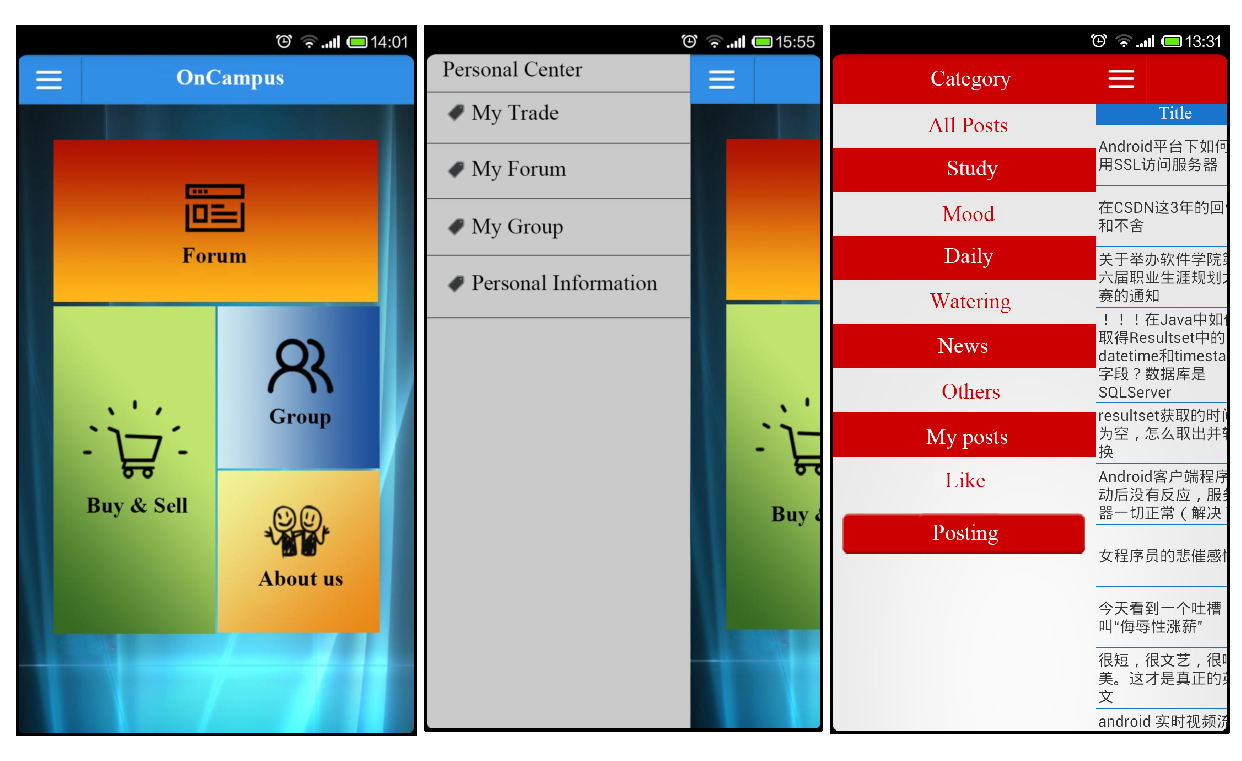
\includegraphics [width=3.5in]{Fig4.pdf}
\caption{The prototype implementation of OnCampus: main interface and "Forum"}
\end{figure}

The "Group" module provides campus with functions of social network which is of great popularity among college student and meets the need of students�� social communication. Circles with various topics can be built up for students to communicate with the users who have similar interest. This helps students to make friends, improve their perception, and broaden their horizons. Personal friends can be added like some instant message systems, and status delivery, share, retweet among circles are supported in this module as well. For example, a user delivery a status that he/she is happy today, everyone within his/her circles will be able to view this, and his/her friends are the ones who have privilege to reply, share, or forward this status.

The "Buy \& Sell" module plays a practical role in campus life for students to exchange their goods. This module is designed to solve the problem of resource waste that students have to throw away their article for daily use or books which are useful and helpful for other students. With "Buy \& Sell", students can release the information about what are not among their necessities and are willing to sell to others. Customers thus will be able to find their needs and complete transactions with the information shown in this module. Users have the rights to view product lists, search certain products, release products offered for sale, and manage his/her on sale product list. Product lists are displayed according to various types of the products, so students can look over a certain type of products with an easy slide on type tabs. Usually the products in these lists will be set as for sale, whereas the product that has been sold can be either marked as fact or deleted from lists as its owner orders.

\begin{figure}[htb]
\centering
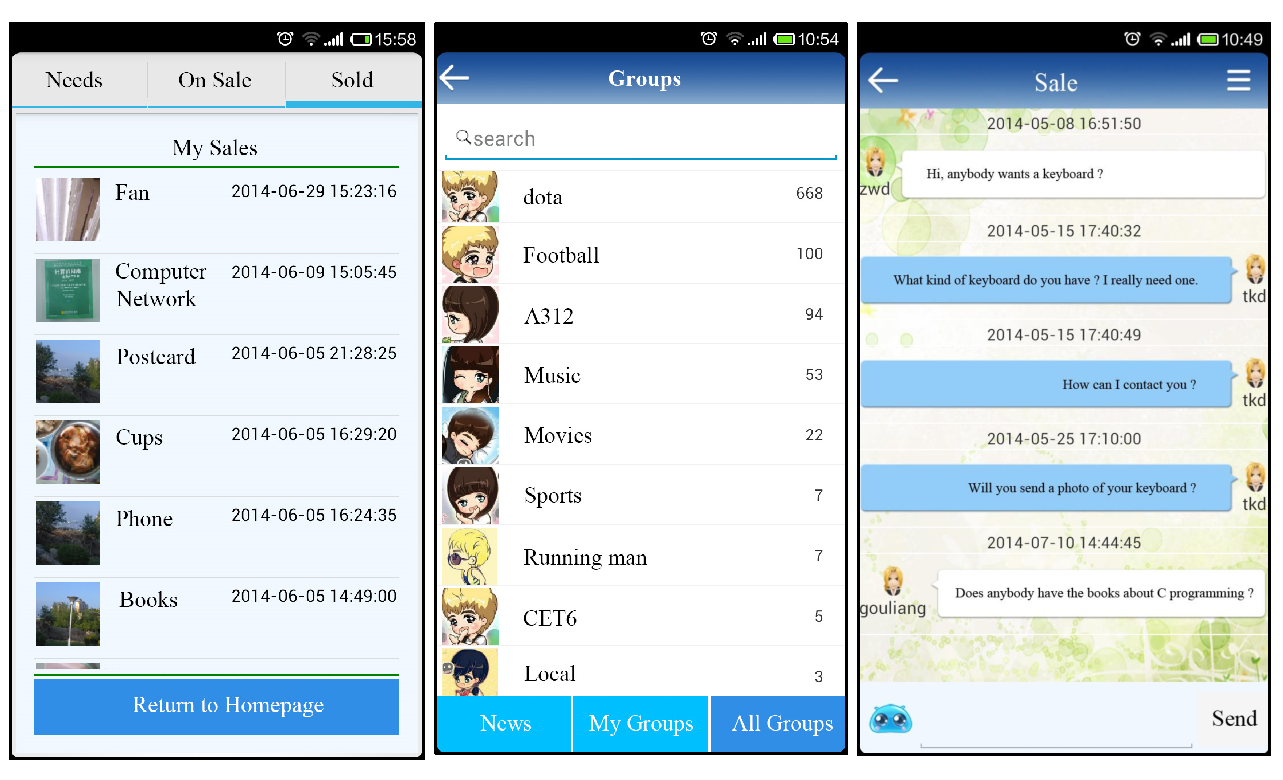
\includegraphics [width=3.5in]{Fig5.pdf}
\caption{The prototype implementation of OnCampus: "Group" and "Buy\&Sell" }
\end{figure}

The "Forum" module is a practical implementation for knowledge sharing, affective interaction and Q \& A. This module is designed to provide a platform for students to share their knowledge, release some news, pour forth their feelings and ask for help. Any register members of OnCampus can read and reply the posts. The owner of the posts can delete, edit, or share his/her posts. They have full privilege to manage it. Everyone here enjoy full freedom of speech.

Particularly speaking, the design and implementation of OnCampus is of great significance. Basically, OnCampus spares no efforts on convenience and efficiency for college students. And practicability of this work can be demonstrated by its wide range of helpfulness for campus situations. For example, Jack is interested in skiing sport very much and wants to find students who have similar interests. One solution is to look for circles with such topics in "Group" module in OnCampus, where holds expected students. And if no such circles can be found, Jack can build up a circle with skiing topic to attract students. Jack will find good friends who have the same hobbies with him in this circle. Another case is that with a new computer keyboard, students would rather prefer to sell the old and unbroken one on the "Buy \& Sell" module to the student who needs it, in an economical and environmental friendly way. Convenience is pursued in university in many scenarios, and OnCampus can be an option at these circumstances.

It can be an intelligent assistant not only because of the practical architecture for college student, but also for its character of energy efficient. LM2C architecture for server is deployed to achieve the energy saving problem for location based service. Specifically speaking, the first time a client connects LSS it receives extra information for following computation of MSS without repeated connection to LSS. This communication mechanism is designed to save energy. And an experiment is conducted to evaluate its performance on three smart phones with same configurations for five times. Phone 1 is set to run no applications to get a standard standby time. Phone 2 runs our prototype OnCampus to calculate location and server information, and Phone 3 runs a controlled prototype without LM2C architecture which communicates with server every time to identify its location. The result of the experiment shows that our architecture has a better performance as three times than the prototype without LM2C architecture.

Besides the substantial services and efficiency, furthermore, it has great potential to make our scheme feasible towards smart campus. Specially speaking, user interests can be revealed when using OnCampus system especially in "Group" module. Data and information will be generated when users interact with the circle member. There is the information of location, user track, proximity, activities and so on. What's more, preference and profile data can be collected when they use the "Buy \& Sell" module and "Forum" module. All of these information has the unpredictable potential to conduct the scheme we introduced above.



\section{Conclusion}

In this paper, we realize the inevitable trend of smart campus. A feasible scheme composed of interests mining, scientific guidance and resources optimizing is proposed towards the construction of smart campus after analyzing the requirements to be satisfied. We summarize the state of art on smart campus. Beyond paralleled development on theory or entity, we design and implement a prototype proven to be efficient based on the proposed scheme.



% use section* for acknowledgement
\section*{Acknowledgment}


\balance
\bibliographystyle{IEEEtran}
\bibliography{OnCampus}

% that's all folks
\end{document}


